%!TEX root = ../thesis.tex

\thispagestyle{myheadings}

\graphicspath{{Body/Figures/ExperimentalOverview/Decay/}{Body/Figures/TrackingFigures/TrackerPics/}{Body/Figures/ExperimentalOverview/Ring/}{Body/Figures/ExperimentalOverview/Accelerator/}{Body/Figures/ExperimentalOverview/Beam/}{Body/Figures/ExperimentalOverview/Auxiliary/}{Body/Figures/MagneticField/}}

\chapter{Principle Techniques of E989}
\label{chapter:E989}

As referenced in \equref{eq:torque}, a particle in a magnetic field will experience a torque which attempts to line up the magnetic dipole moment of the particle with the external field. Because of this, in a dipole field a particles spin will turn at the precession frequency \cite{Jackson}
        \begin{align} \label{eq:ws}
            \vec{\omega}_{s} = -g\frac{q}{2m}\vec{B} - (1-\gamma)\frac{q}{\gamma m}\vec{B},
        \end{align}
where as before $m$ is the particles mass, $q = \pm e$ where $e$ is the positive elementary charge, \g is the g-factor, $\gamma$ is the Lorentz relativistic factor, and $B$ is an external magnetic field. The first term is the usual Larmor frequency and the second term is a relativistic correction to the precession frequency called Thomas precession \cite{Jackson}. Similarly, a particle with some momentum will orbit at the cyclotron frequency
        \begin{align} \label{eq:wc}
            \vec{\omega}_{c} = -\frac{q}{\gamma m}\vec{B}.
        \end{align}
By taking the difference between these two frequencies we arrive at the ``spin difference frequency''
        \begin{align} \label{eq:wasimple}
            \vec{\omega}_{a} = \vec{\omega}_{s} - \vec{\omega}_{c} = -\frac{g-2}{2}\frac{q}{m}\vec{B} = - a \frac{q}{m}\vec{B},
        \end{align}
a frequency that is directly proportional to anomaly $a$. If $g = 2$ as in a Dirac theory, then the particles spin would turn at the same rate as the momentum vector, and this spin difference frequency \wa would be identically zero. If this spin difference frequency for a muon and the external magnetic dipole field can be measured, then the anomalous magnetic moment of the muon \amu can be measured. 

As will be detailed below in \secref{sec:MagneticField}, the measurement of the magnetic field is related to the Larmor precession frequency of free protons in water 
        \begin{align} \label{eq:wp}
            \omega_{p} = -g_{p} \frac{e}{2m_{p}} B,
        \end{align}
where $g_{p}$ and $m_{p}$ are the g-factor and mass of the proton respectively. Replacing $B$ and solving for \amu, we arrive at 
        \begin{align} \label{eq:amu}
            a_{\mu} = \frac{g_{p}}{2} \frac{\omega_{a}}{\omega_{p}} \frac{m_{\mu}}{m_{p}}.
        \end{align}
Using the magnetic moment formulas for the proton, electron, and muon as shown in \equref{eq:magneticmoment}, \equref{eq:amu} can be transformed to either of the following consistent equations:
        \begin{equation} 
        \begin{aligned} \label{eq:amuratios}
            a_{\mu} &= \frac{g_{e}}{2} \frac{\omega_{a}}{\omega_{p}} \frac{m_{\mu}}{m_{e}} \frac{\mu_{p}}{\mu_{e}} \\ 
            a_{\mu} &= \frac{\omega_{a}/\omega_{p}}{\lambda - \omega_{a}/\omega_{p}}
        \end{aligned}
        \end{equation}
Here the $p$, $e$, and $\mu$ subscripts stand for the relevant quantities for the proton, electron, and muon respectively. In the second equation $\lambda = \mu_{\mu}/\mu_{p}$. As mentioned before the electron g-factor $g_{e}$ has been measured to extremely high precision, 0.26 ppt \cite{ElectronMDM,CODATA}. The muon-electron mass ratio $m_{\mu}/m_{e}$ and muon-proton magnetic moment ratio $\lambda$ have been measured to 22 ppb \cite{CODATA,MuoniumHyperfine}. Finally the proton-electron magnetic moment ratio $\mu_{p}/\mu_{e}$ has been measured to 3 ppb \cite{CODATA}. The errors on these terms are small compared to the target uncertainty for E989 of 140 ppb, the measurement of which now comes down to measuring the ratio $\omega_{a}/\omega_{p}$. 


\section{Measuring \texorpdfstring{\wa}{wa}}
\label{section:WaIntro}

How can \wa for muons be measured? The answer lies with two key points in the dynamics of muon decay. Positive muons decay to a positron and two neutrinos, as shown in \figref{fig:mudecay}. The first point is that because of the parity violating nature of the weak interaction, the decay positron will be preferentially emitted right-handed, with its spin directed in the same direction as its momentum \cite{Bucksbaum}. The second key point is that angular momentum must be conserved. Consider the most extreme examples of maximum and minimum energy positrons as shown in \figref{fig:MuonDecayImproved}. In the muon rest frame, decay positrons with maximum energy will be emitted opposite to the two neutrinos. Since neutrinos and anti-neutrinos must be left and right-handed respectively, thus having their spins anti-parallel and parallel to their momentum, by the law of conservation of angular momentum the positron must have its spin be parallel to the spin of the muon at the time of the decay. By the opposite argument, decay positrons emitted with minimum energy such that the neutrinos are ejected opposite to one another must have their spins be anti-parallel to that of the muon at the time of decay. These two points combined together means that higher energy decay positrons will preferentially be emitted in directions parallel to the muon spin at the time of decay, while lower energy decay positrons will preferentially be emitted in directions anti-parallel to the muon spin at the time of the decay. 

\begin{figure}[]
\centering
    \subcaptionbox{$\mu^{+}$ decay through a $W^{+}$ boson to a positron, muon anti-neutrino, and an electron neutrino. This is the dominant decay mode.
    \label{fig:mudecay}}
    {
    \centering
        \begin{tikzpicture}[baseline=(o.base)]
        \begin{feynhand}
        \large
        \setlength{\feynhandlinesize}{1pt}
        \vertex [dot] (o) at (0,0);
        \vertex (a) at (-2,0) {$\mu^{+}$}; 
        \vertex (b) at (1.5,1.5) {$\overline \nu_{\mu}$}; 
        \vertex (c) at (1.5,-1.5);
        \vertex (d) at (3,0) {$\nu_{e}$};
        \vertex (e) at (3,-3) {$e^{+}$};
        \propag [anti fermion] (a) to (o);
        \propag [fermion] (b) to (o);
        \propag [boson] (o) to [edge label' = $W^{+}$] (c);
        \propag [fermion] (c) to (d);
        \propag [anti fermion] (c) to (e);
        \end{feynhand}
        \end{tikzpicture} 
    }
    \hspace{10mm}
    \subcaptionbox{$\pi^{+}$ decay through a $W^{+}$ boson to a $\mu^{+}$.
    \label{fig:pidecay}}
    {
    \centering
        \begin{tikzpicture}[baseline=(o.base)]
        \begin{feynhand}
        \large
        \setlength{\feynhandlinesize}{1pt}
        \vertex [dot] (o) at (0,0);
        \vertex (a) at (-1.5,1.5) {$u$}; 
        \vertex (b) at (-1.5,-1.5) {$\overline d$}; 
        \vertex (c) at (2,0);
        \vertex (d) at (3.5,1.5) {$\mu^{+}$};
        \vertex (e) at (3.5,-1.5) {$\nu_{\mu}$};
        \propag [fermion] (a) to (o);
        \propag [anti fermion] (b) to (o);
        \propag [boson] (o) to [edge label = $W^{+}$] (c);
        \propag [anti fermion] (c) to (d);
        \propag [fermion] (c) to (e);
        \end{feynhand}
        \end{tikzpicture}  
    }
\caption[Feynman diagrams for muon and pion decay]{Feynman diagrams for muon (left) and pion (right) decay.}    
\label{fig:DecayDiagrams}
\end{figure}

\begin{figure}[]
    \centering
    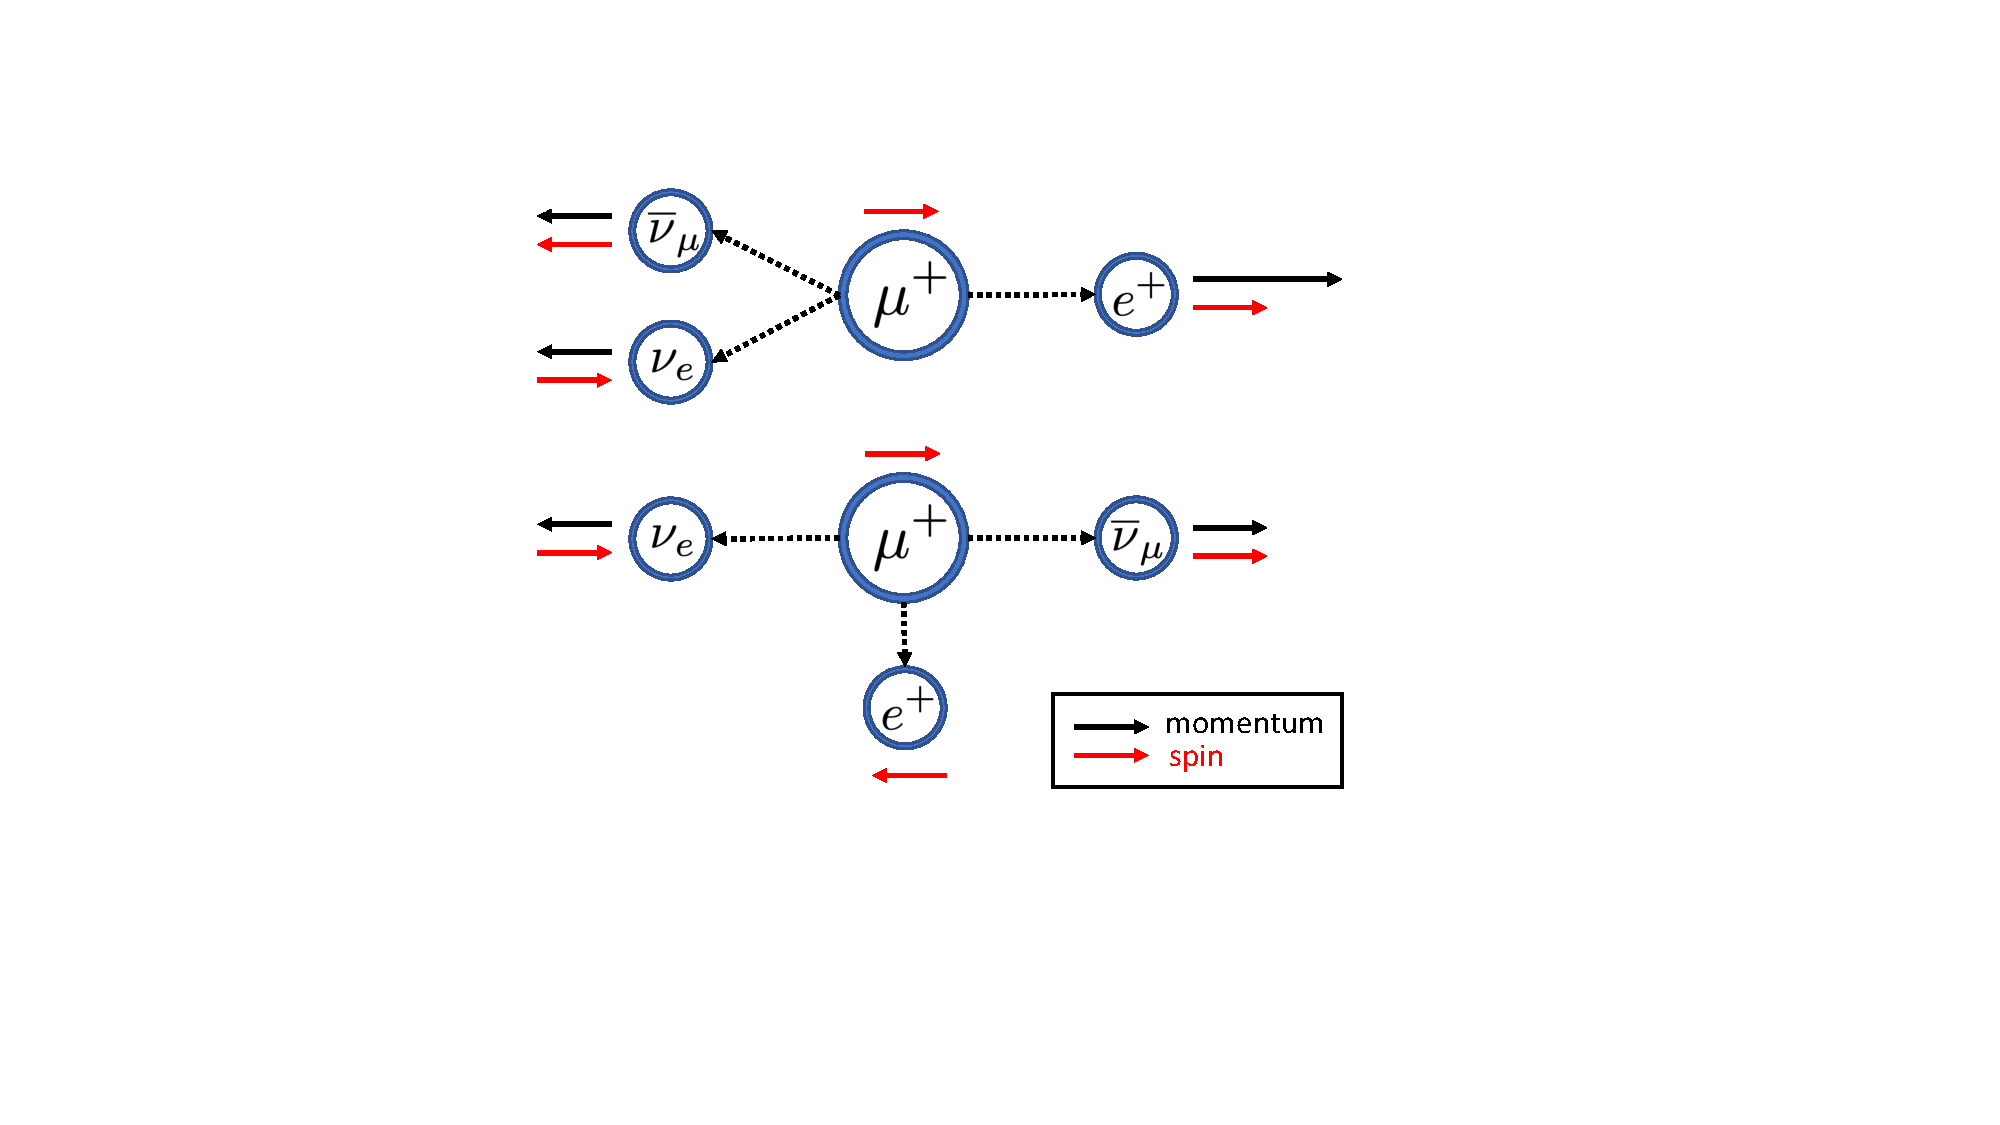
\includegraphics[width=0.6\textwidth]{MuonDecayImproved}
    \caption[Muon decay pictures for maximum and minimum energy decay positrons]{Muon decay pictures for maximum and minimum energy decay positrons. Due to the conservation of angular momentum and the single possible helicity states of the decay neutrinos, the spin of the decay positron is exactly parallel to the spin of the muon at the time of the decay for maximum energy decay positrons (top), or anti-parallel for minimum energy decay positrons (bottom).}
    \label{fig:MuonDecayImproved}
\end{figure}


This correlation between the emitted direction of the decay positron and the spin of the muon is the signature needed to measure \wa. By placing an ensemble of polarized muons within a magnetic storage ring, those muons will orbit at the cyclotron frequency and their spins will precess at the Larmor frequency. As they go around the ring they will decay to positrons whose energy and decay directions contain information about the spin of the muon. The differential decay distribution in the muon rest frame is described by \cite{Bucksbaum}
        \begin{align} \label{eq:diffdecaydist}
            dP(y, \theta) \propto N(y)[1 \pm A(y)\cos(\theta)]dy d\Omega,
        \end{align}
where $y=E/E_{max}$ is the energy fraction of the positron, $\theta$ is the angle between the spin of the muon and the momentum of the positron $\cos^{-1}(\hat{p} \cdot \hat{s})$, and the $\pm$ stands for the positive and negative muon respectively. $N(y)$ is the number distribution of decay positrons and $A(y)$ is the so called 'asymmetry' encoding the preferred positron decay direction. Here the energy of the positron is assumed to be much greater than its mass. The number distribution and asymmetry are given by \cite{Bucksbaum}
        \begin{align}
            N(y) &= 2y^{2}(3-2y^{2}), \label{eq:Nmrf} \\
            A(y) &= \frac{2y-1}{3-2y}, \label{eq:Amrf}
        \end{align}
and are shown in \figref{fig:NA2mrf}. 

\begin{figure}[]
\centering
    \begin{subfigure}[]{0.45\textwidth}
        \centering
        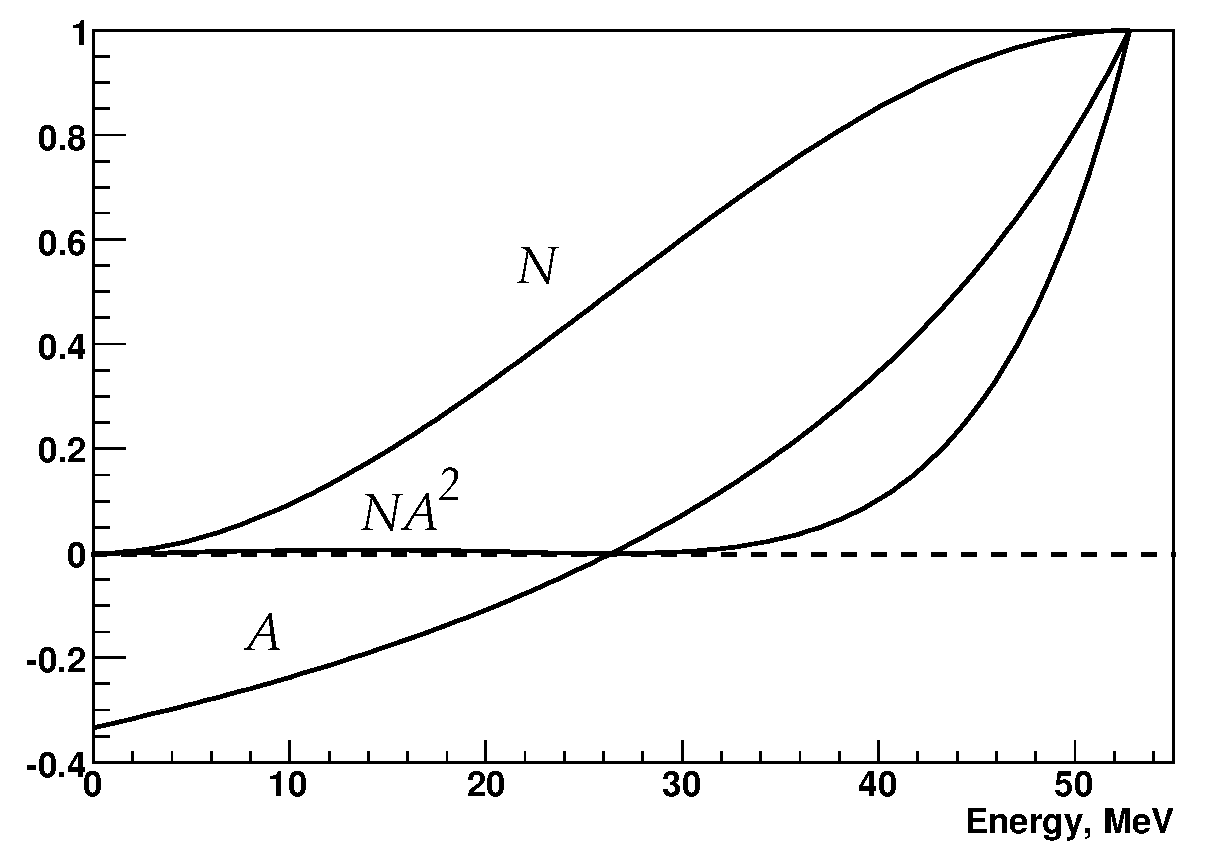
\includegraphics[width=\textwidth]{NA_mrf}
        \caption{Muon rest frame}
    \label{fig:NA2mrf}
    \end{subfigure}%
    \hspace{1cm}
    \begin{subfigure}[]{0.45\textwidth}
        \centering
        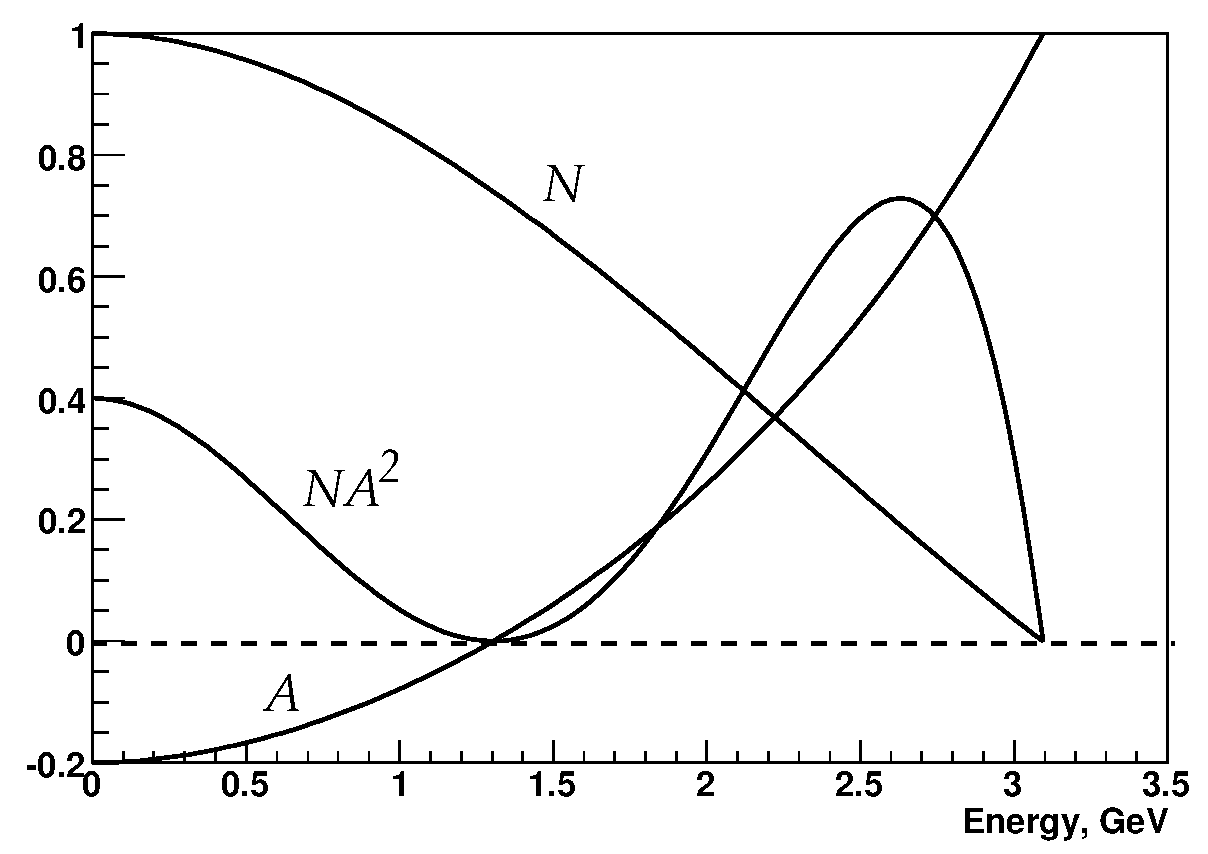
\includegraphics[width=\textwidth]{NA_lab}
        \caption{Lab frame}
    \label{fig:NA2lab}    
    \end{subfigure}
\caption[Number distribution and asymmetry for muon decay in the muon rest frame and lab frame]{Decay number distribution $N$ and asymmetry $A$ in the muon rest frame (left) and in the lab frame (right) as a function of positron energy with a maximum positron energy of 3.1 \GeV.}
\label{fig:NA2}
\end{figure}

In the lab frame for high energy positrons, nearly all positrons will be emitted parallel to the muon momentum, which makes it challenging to select purely on the decay angle of the positron. That's not a problem though, as we already know that decay positrons with higher energies will be emitted in directions parallel to the muon spin at the time of decay. Essentially, the energy distribution of detected positrons for high energies is modulated by \wa, or $\theta = \omega_{a}t + \phi$. The number of detected positrons at some time and energy in the lab frame for some initial number $N_{0}$ of muons can then be described by
        \begin{align}
            N_{d}(t, E) = N_{0}(E) \cdot e^{-t/\gamma\tau_{\mu}} \cdot [1 + A(E) \cos(\omega_{a}t+\phi(E))],
        \end{align}
where the $d$ subscript stands for 'detected,' the muons are decaying at a lifetime of $\gamma\tau_{\mu}$, and all the relevant parameters are energy dependent. Here $N_{0}(E)$ and $A(E)$ have been transformed from Equations~\ref{eq:Nmrf} and \ref{eq:Amrf} to the lab frame,
        \begin{align}
            N_{0}(E) &\propto (y-1)(4y^{2}-5y-5), \label{eq:Nlab} \\
            A(E) &= \frac{-8y^{2}+y+1}{4y^{2}-5y-5}, \label{eq:Alab}
        \end{align}
where as a reminder $y=E/E_{max}$. Here the polarization of the muons is assumed to be unity. These are shown in \figref{fig:NA2lab}. To increase the amount of statistics, all positrons above some energy threshold cut $E_{th}$ can be taken as the observable,
        \begin{align} \label{eq:5parfunc}
            N_{d}(t, E_{th}) = N_{0}(E_{th}) \cdot e^{-t/\gamma\tau_{\mu}} \cdot [1 + A(E_{th}) \cos(\omega_{a}t+\phi(E_{th}))],
        \end{align}
where the number and asymmetry of the detected positrons is now calculated by simply integrating Equations~\ref{eq:Nlab} and \ref{eq:Alab} from $y_{th}$ to 1,
        \begin{align}
            N_{0}(E_{th}) &\propto (y_{th}-1)^{2}(-y_{th}^{2}+y_{th}+3), \label{eq:Nth} \\
            A(E_{th}) &= \frac{y_{th}(2y_{th}+1)}{-y_{th}^{2}+y_{th}+3}, \label{eq:Ath}
        \end{align}
where $y_{th}=E_{th}/E_{max}$. By fitting \equref{eq:5parfunc}, \wa can be extracted. An sample of data adhering to \equref{eq:5parfunc} is shown in \figref{fig:gm2wiggle}.


\begin{figure}[]
    \centering
    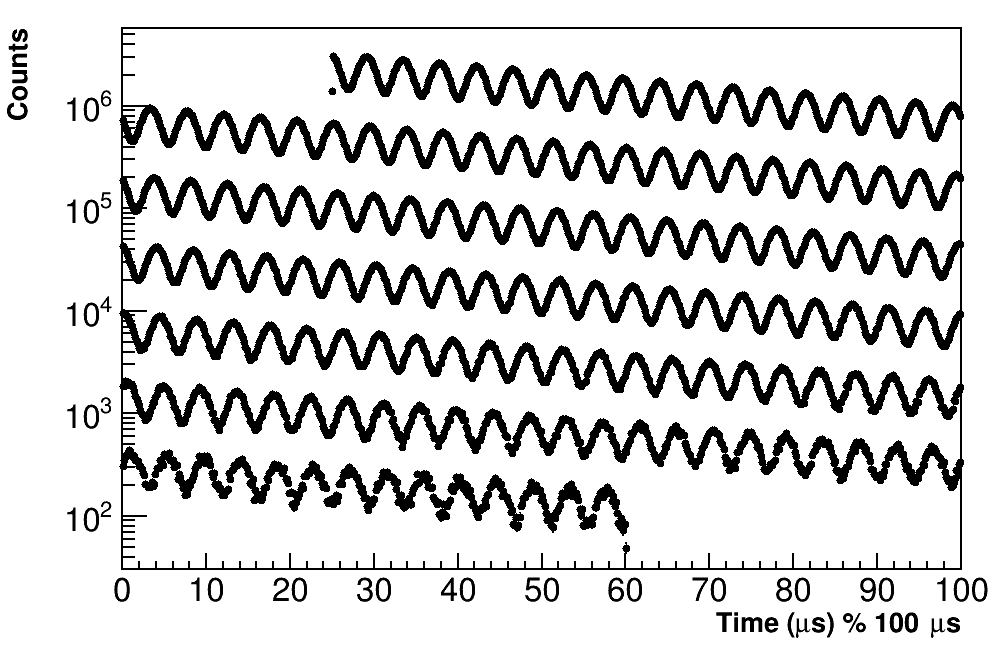
\includegraphics[width=0.9\textwidth]{gm2wiggle}
    \caption[\gmtwo wiggle example]{The number of detected positrons above some energy threshold ($y \sim 0.55$) as a function of time. The time axis is wrapped around every \mus{100}.}
    \label{fig:gm2wiggle}
\end{figure}



\section{Measuring the magnetic field}
\label{sec:MagneticField}


In order to measure the magnetic moment of the muon to 140 ppb, the field needs to be both highly uniform, and measured to extreme precision. The E989 goal for the field measurement is 70 ppb. As shown in \equref{eq:amuratios} the measurement of the magnetic field has equal weight to that of the precession frequency. A cross-section of the magnetic ring is shown in \figref{fig:MagnetCrossSection}. The muons live within a $\SI{9}{cm^{2}}$ diameter cylindrical storage region at the center of the magnetic field. This corresponds to an approximately $\SI{0.28}{m^{3}}$ or $\SI{10}{ft^{3}}$ total volume around the inside of the ring. The magnetic field is made uniform by manipulating many magnetic `knobs' built into the \gmtwo storage ring, including the main magnet current, pole pieces, wedges, top hats, and thousands of small magnetic shims placed around the storage region. There is also an active feedback system which stabilizes the magnetic field over time. The shimming of the field to high precision, to an RMS (root mean square) of approximately $\SI{25}{ppm}$, was a long process of fine tuning over the course of many months that was undertaken by many members of the field team.

\begin{figure}[]
    \centering
    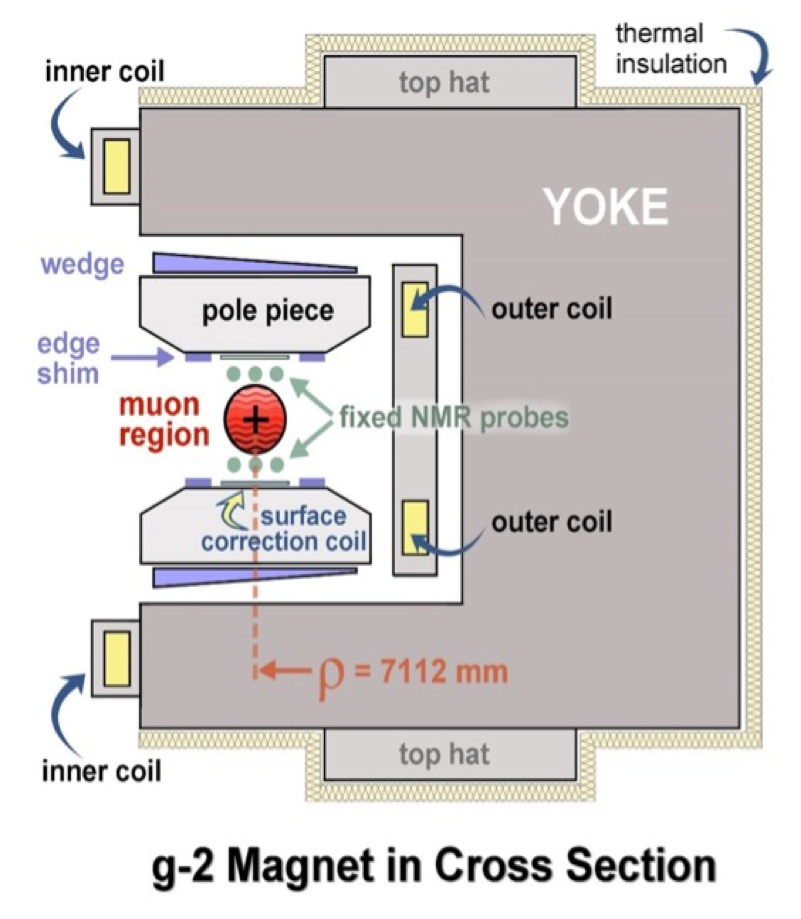
\includegraphics[width=0.9\textwidth]{MagnetCrossSection}
    \caption[Magnet cross section]{Cross-section of the \gmtwo magnet. The muons live in the storage region. This is surrounded by many magnetic features of the magnet which allow for sub ppm level tuning of the magnetic field.}
    \label{fig:MagnetCrossSection}
\end{figure}


Measuring the magnetic field comes down to measuring $\omega_{p}$ as shown in \equref{eq:wp}. This is because the magnetic field measurement is made using a pulsed nuclear magnetic resonance technique (NMR). NMR was chosen as it provides a field measurement precision on the order of 10 ppb with negligible statistical uncertainty \cite{TDR}. NMR probes work by rotating the magnetization of a sample of protons in some fluid, typically water or petroleum jelly, and then measuring the relaxation time or free-induction decay (FID) signal of the proton spins. The magnetization of the protons will relax back to equilibrium with the external field as the spins of the protons precess at the Larmor frequency and interact with local magnetic field gradients or inhomogeneities. Pickup coils are located around the sample which both deliver the pulse to rotate the proton sample magnetization and measure the FID signal. An example of an FID signal is shown in \figref{fig:FID}.

\begin{figure}[]
    \centering
    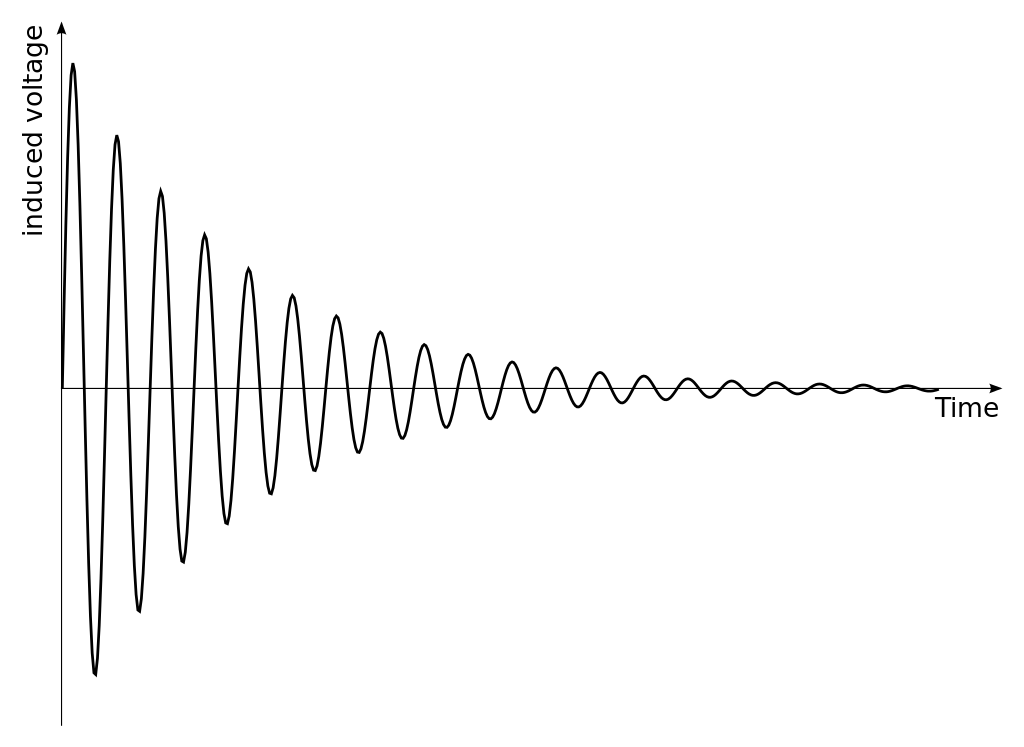
\includegraphics[width=0.6\textwidth]{Nmr_fid_good_shim_EN}
    \caption[FID signal]{An example FID signal. The current picked up in the coils around the proton sample will oscillate as the spins precess around the main magnetic field, and decay as the spins return to alignment with the external field.}
    \label{fig:FID}
\end{figure}

Technically, it is not solely $\omega_{p}$ that needs to be measured. What really matters is the average magnetic field that the muons see, or the time-averaged spatially-weighted magnetic field. The scheme devised to measure this is two-fold. First, the magnetic field in the storage region where the muons live is measured by a trolley which drives around the inside of the ring. This trolley holds 17 NMR probes and measures the field at approximately 6000 locations around the inside of the ring. Because however the trolley cannot be in the beam path when the muons are present in the ring, during data taking it is pulled out of the way and the field is instead measured by 378 fixed NMR probes located in the high magnetic field region, but just outside the storage region. The prescription is that the fixed probes measure the field at all times, the storage ring field is measured every few days by the trolley probes, and the two are interpolated. In this way the magnetic field can be mapped over time and over the space that the muons live in. A preliminary sample of the azimuthally-averaged magnetic field measured with trolley and fixed probes is shown in \figref{fig:AverageMagneticField}.

\begin{figure}[]
    \centering
    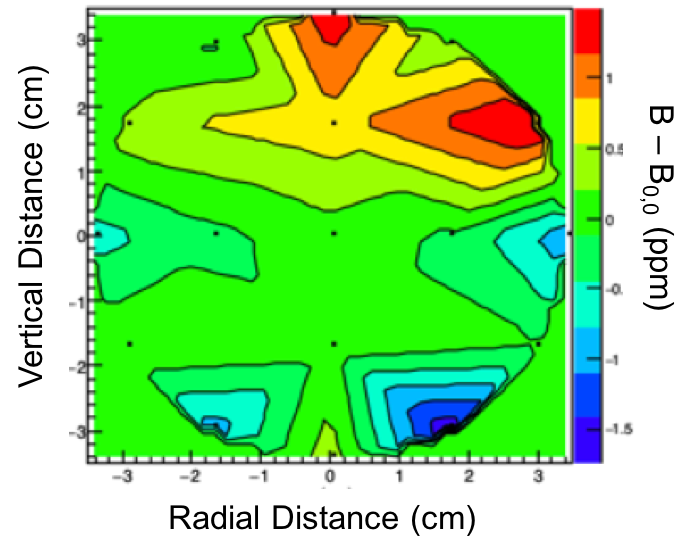
\includegraphics[width=0.6\textwidth]{AverageMagneticField}
    \caption[Azimuthally averaged magnetic field sample]{A sample of the azimuthally-averaged magnetic field within the storage region. The contours are normalized to the center value of the field. The scale of the field differences is approximately $\pm 1$ ppm. The dots in the picture correspond to the location of the trolley probes. \textbf{Update this picture later on and find out what the time averaging is.}}
    \label{fig:AverageMagneticField}
\end{figure}


Lastly, it is the free proton precession frequency in the field that is of interest, but the frequency that the probes measure will be different due to the molecular properties of the proton sample as well as the material properties of the probe itself. The frequency that the probes measure can be re-casted as 
        \begin{align} \label{eq:wpprobe}
            \omega_{p,\text{probe}} = \omega_{p,\text{free}}(1 - \sigma(\text{H\textsubscript{2}O, T}) + \delta_{b} + \delta_{p} + \delta_{s}),
        \end{align}
where $\sigma(\text{H\textsubscript{2}O, T})$ is the temperature dependent diamagnetic shielding of protons in a water molecule, and the $\delta$'s come from corrections due to the bulk susceptibility of the water sample, paramagnetic impurities in the water sample, and the magnetic effects of the probe itself, respectively \cite{TDR}. In order to correct for these effects two additional special probes are used, both of which live in a single section of the ring which has been shimmed to extra uniformity. The first is a calibration probe which measures the free proton precession frequency at the center of the storage region corresponding to the placement of the central trolley probe. The calibration probe is made of materials in order to reduce the effects in \equref{eq:wpprobe} and has been characterized in other test magnets. The second special probe is called the `plunging probe.' This probe lives inside the vacuum chamber and drops into the storage region to measure the field at each of the 17 trolley probe locations, using a three dimensional motion system. By using these two probes, the calibration for the free proton precession frequency can be transmitted to each of the trolley probes, providing for the needed measurement inside the storage region of the magnetic field. This calibration procedure is estimated to take up about half of the target systematic uncertainty of 70 ppb at 35 ppb.


Other pieces of the systematic uncertainty include the absolute calibration of the calibration probe, the trolley measurements, the interpolation to the fixed probes, the uncertainty relative to the muon distribution, and others such as time dependent external magnetic fields. See \tabref{tab:magneticfielduncertainties} When all is said and done, the measurement of the magnetic field is a complex and continuous process that is done in parallel to the measurement of \wa throughout data taking. 


\begin{table}[]
\centering
\setlength\tabcolsep{10pt}
\renewcommand{\arraystretch}{1.2}
\begin{tabular*}{.8\linewidth}{@{\extracolsep{\fill}}lc}
  \hline
    \multicolumn{2}{c}{\textbf{Magnetic Field Measurement Uncertainties}} \\
  \hline\hline
    Source of uncertainty & E989 Goal (ppb) \\
  \hline
    Absolute calibration of standard probe & 35 \\
    Calibration of trolley probes & 30 \\
    Trolley measurements & 30 \\
    Fixed probe interpolation & 30 \\
    Muon distribution weighted average & 10 \\
    Time dependent external fields & 5 \\
    Others & 30 \\
  \hline
    Quadrature sum & 70 \\
  \hline 
\end{tabular*}
\caption[Uncertainties in the magnetic field measurement]{Systematic errors in the magnetic field measurement. Unlisted sources of error include the measurement of higher field multipoles, trolley temperature and power supply voltage response effects, and eddy currents from the kicker, among others.}
\label{tab:magneticfielduncertainties}
\end{table}



\section{Production of polarized muons}
\label{sec:Accelerator}

As explained previously, the number of high energy positrons detected depends on the muon spin at the time of decay. In order for this detected quantity to mean anything, the muon spins themselves need to be highly polarized. Using the same parity-violation and spin momentum conservation logic as expounded upon in muon decay, it is determined that pion decay produces muons that are 100\% polarized in the pion rest frame, due to the pion having zero spin. The Feynman diagram for this decay is shown in \figref{fig:pidecay}. It's also important to note that pions decay to muons with over 99\% branching ratio due to the parity violating nature of the weak interaction, and thus a preference for the heavier muon over the electron. These two facets of pion decay are used to construct polarized muon beams. 

In order to measure \gmtwo to high precision, a very large number of positrons need to be detected, and hence a large number of highly polarized muons injected into the storage ring. The BNL E821 experiment observed on the order of 10 billion positrons above threshold, and its final result was statistics limited. In order to reach the goal of 140 ppb, 20 times that number of statistics needs to be gathered. The only facility in the world that can produce such a high number of polarized muons is Fermilab. 

\begin{figure}[]
    \centering
    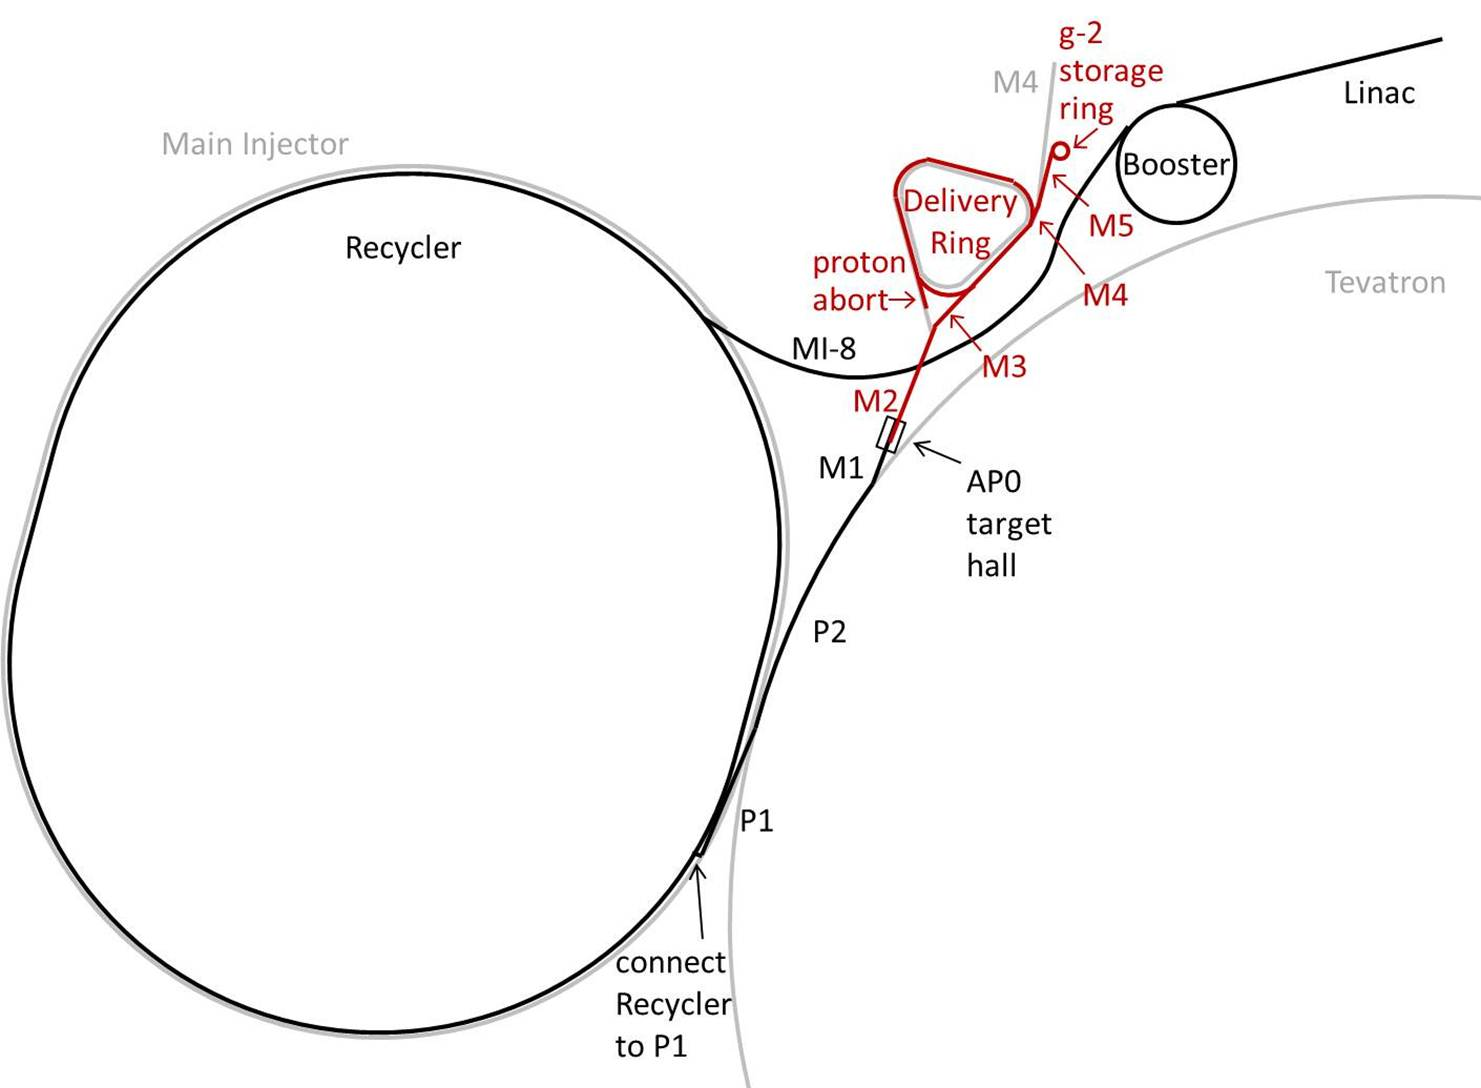
\includegraphics[width=1\textwidth]{accel_layout}
    \caption[Fermilab accelerator layout for muon delivery to E989]{Plotted is the layout of accelerator beam-line components Fermilab uses to provide polarized muons to E989. Protons start in the Linac, traverse around the Booster and then Recycler, and are converted to pions at AP0. The pions are gathered and then decay away to muons in the Delivery Ring before being sent to the \gmtwo storage ring. Figure taken from \refref{TDR}.}   
    \label{fig:accelerator}
\end{figure}

The Fermilab accelerator complex produces polarized muons for E989 in a number of stages. A map of the various relevant accelerator beam-line components is shown in \figref{fig:accelerator}. Details of the full accelerator production of polarized muons can be found in \refref{Stratakis:2017uci}, and here will be given a summary of the process. First, protons are generated and accelerated in a linear accelerator. They are transported to a small circular ring called the ``booster,'' which accelerates them up to 8 \GeV and batches them together. A single booster batch contains on the order of $\SI{4e12}{protons}$. The protons are then injected into a ring called ``recycler,'' which re-bunches them into four separate bunches of $\SI{1e12}{protons}$, each with a time width of approximately $\SI{120}{ns}$. (This is less than the cyclotron period of the storage ring of 149 ns.) This rebunching process is done in order to reduce the level of pileup in the \gmtwo detectors, see \secref{sub:calosystematics}. For a single accelerator supercycle of $\SI{1.4}{s}$, E989 recieves four booster batches of particles corresponding to sixteen bunches at an average rate of $\SI{11.4}{Hz}$, with the time separation between bunches greater than $\SI{10}{ms}$. The timing structure is shown in \figref{fig:pulsetrain}. The sets of eight bunches are sometimes referred to as pulses, and the gathered data is tagged by which bunch or pulse it originates from. Depending on the accelerator requirements of other experiments, this timing structure is modified appropriately though it is relatively constant.

\begin{figure}[]
    \centering
    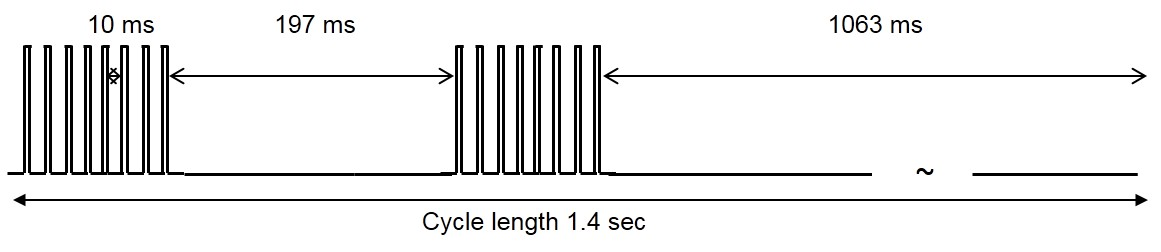
\includegraphics[width=1\textwidth]{accel_pulsetrain}
    \caption[Fermilab accelerator pulse train]{General timing structure of beam pulses sent to E989.}   
    \label{fig:pulsetrain}
\end{figure}


Each bunch is selected one at a time and sent to a target hall, where the bunch is directed on to an Inconel target. This Inconel target is made up of a nickel and iron alloy optimized for producing a large number of pions with a small momentum spread, approximately $\SI{1e-5}{\pi^{+}/\text{POT}}$ with $|dp/p| < 2 \%$ \cite{Stratakis:2017uci}. The resulting pions are focused just after production by a lithium lens. This lithium lens is a $\SI{1}{cm}$ radius and $\SI{15}{cm}$ long piece of lithium designed to carry high current which provides a radial focusing effect for particles passing lengthwise down the cylinder \cite{LiLens}. A pulsed magnet just after the lithium lens is then used to select pions at $\SI{3.115}{\GeV}$.

In a pion beam the highest and lowest energy decay muons are polarized. The pion beam and any residual protons or secondaries are injected into another ring called the ``delivery ring''. By the time the pions have gotten to the delivery ring, most of them have decayed to muons. The delivery ring is used to both hold the beam until the remaining pions decay, which takes about four turns, and to select the polarized muons \cite{Stratakis:2017uci}. Forward emitted polarized muons are momentum selected at $\SI{3.094}{\GeV}$ with $\Delta p / p = 2\%$. The remaining muons, protons, and other secondary particles are separated and re-routed to a beam dump which reduces the contamination in the final polarized muon beam. This polarized muon beam is then sent to the \gmtwo building where it passes through four magnetic quadrupole focusing magnets before being injected into the storage ring.




\section{Injection of muons}
\label{sec:injection}


The injection of the muon beam into the \gmtwo storage ring is a specialized process. In order to measure the magnetic field to the precision described in \secref{sec:MagneticField}, the \gmtwo storage ring must be a single monolithic magnet with no end effects. This prohibits the usual design of separated magnetic elements through which the muons might be injected. Therefore we use a specialized magnet called the ``Superconducting Inflector'' magnet, or just inflector. This inflector is placed just after a bored out tunnel in the storage ring magnet, on the inside of the C shape. See \figref{fig:injectionpoint} for a view of the injection point. The inflector has a very tight $\SI{18}{mm}$ wide by $\SI{56}{mm}$ high aperture through which the muons must pass down its $\SI{1.7}{m}$ length. The inflector is made up of superconducting coils wrapped in a double cosine theta design around an aluminum mandrel \cite{inflector}. See \figref{fig:inflector}. This design serves to contain the majority of the inflector magnet field, while eliminating the the storage ring field for the muons passing down its length, such that they are not lost due to motion induced by said field. The inflector is contained within a superconducting shield which traps the fringe field of the inflector such that the storage ring magnet field is unaffected. As shown in \figref{fig:inflector}, both sides of the inflector are closed such that an appreciable fraction of muons are lost due to multiple scattering before being injected into the ring. Approximately 2\% of injected muons are stored with $\Delta p / p = 0.1\%$ centered around $\SI{3.094}{\GeV}$. A new inflector magnet is being designed with open ends in order to increase the muon flux for future runs of \gmtwo \cite{TDR}.


\begin{figure}[]
    \centering
    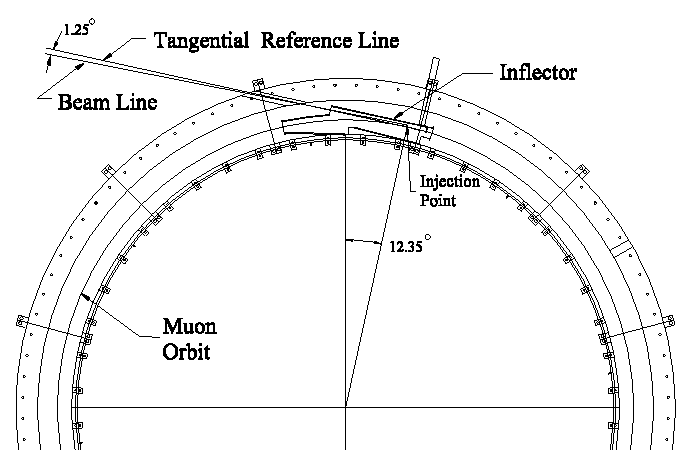
\includegraphics[width=.7\textwidth]{injectionpoint}
    \caption[Muon injection point through inflector]{Shown is a plan view of the inflector and injection point into the storage ring \cite{inflector}.}   
    \label{fig:injectionpoint}
\end{figure}

\begin{figure}[]
\centering
    \begin{subfigure}[t]{0.45\textwidth}
        \centering
        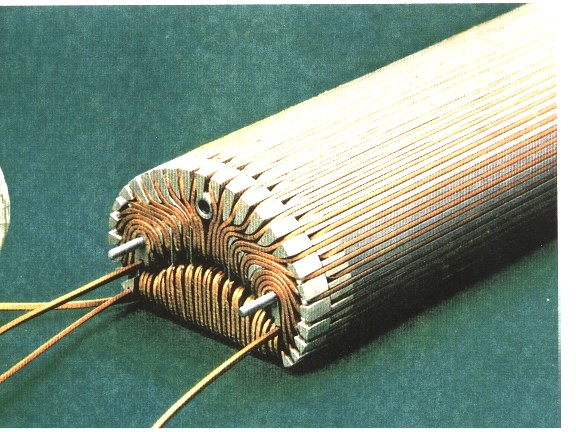
\includegraphics[width=\textwidth]{inflector_closed}
        \caption{End view of the inflector.}
    \end{subfigure}%
    \hspace{1cm}
    \begin{subfigure}[t]{0.45\textwidth}
        \centering
        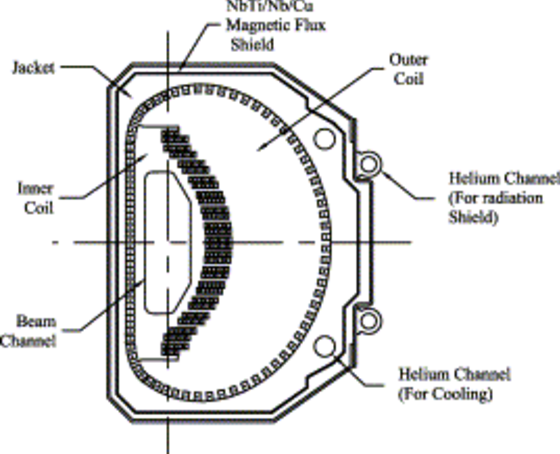
\includegraphics[width=\textwidth]{inflectorcrosssection}
        \caption{Cross section view of the inflector.}
    \end{subfigure}
\caption[Superconducting inflector magnet]{The inflector magnet (left) and a cross section view of the inflector windings and associated shield (right) \cite{inflector}.}
\label{fig:inflector}
\end{figure}



\section{Storage of muons}
\label{sec:Storage}

\begin{figure}[]
    \centering
    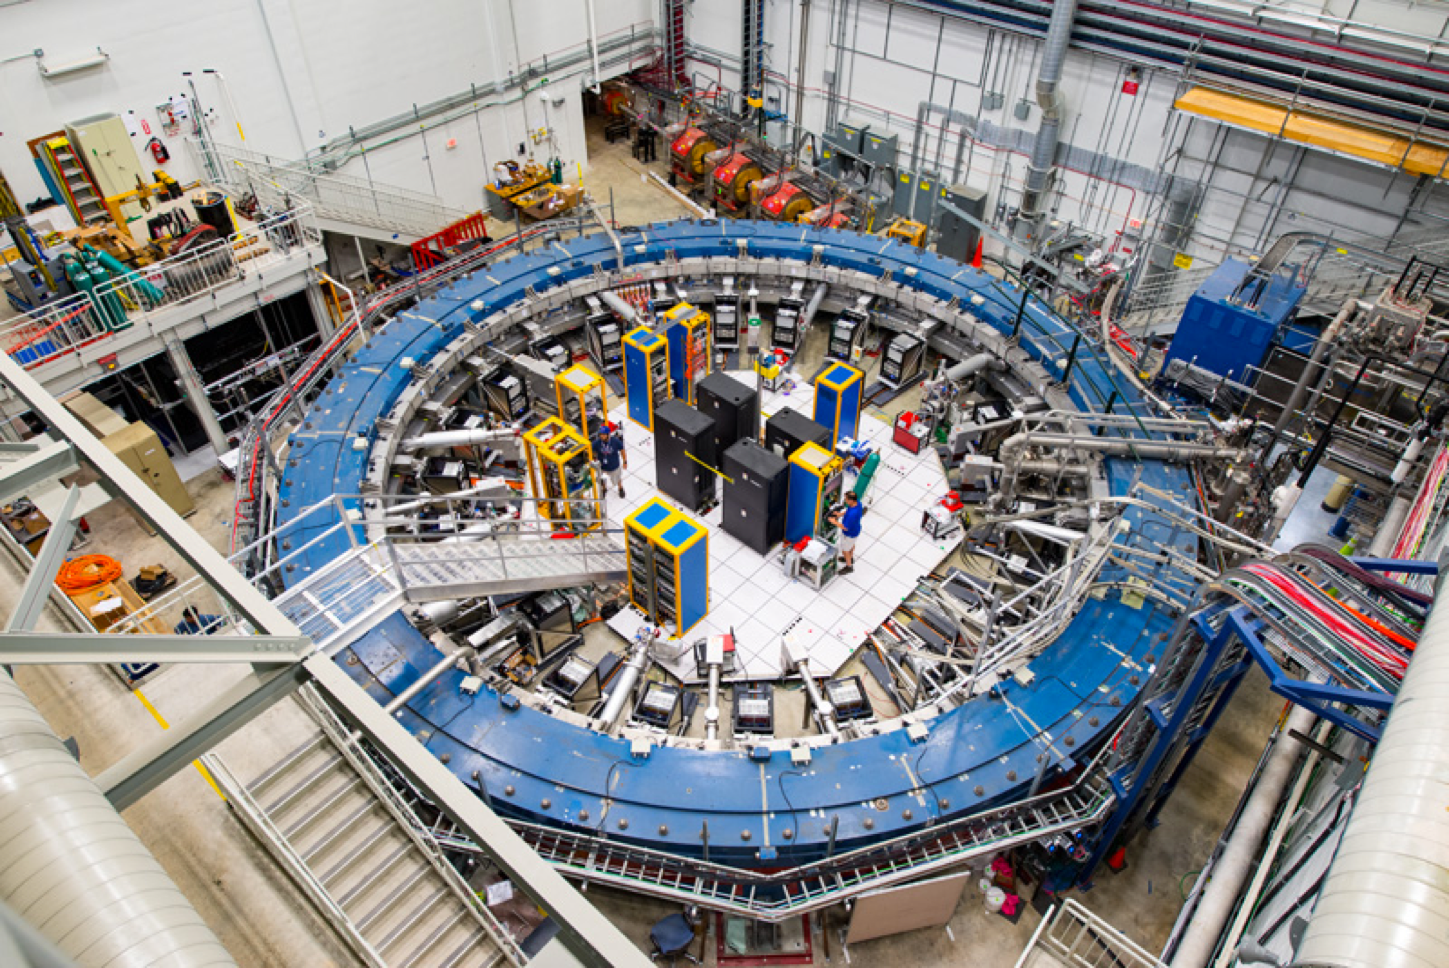
\includegraphics[width=1\textwidth]{ring}
    \caption[The \gmtwo experiment]{Shown is a picture of the \gmtwo experiment. The blue painted storage ring can be seen to surround a variety of detectors and electronics. Muons come in at the top of the picture through a serious of magnetic quadrupoles from the accelerator and are injected into the ring, where they orbit in a clockwise direction. There are some people located inside the ring which gives a sense of scale to the picture.}   
    \label{fig:ring}
\end{figure}


The E989 experiment and storage ring are shown in \figref{fig:ring}. Approximately 10,000 muons are stored in the \gmtwo ring at a time, corresponding to a single fill. The $\SI{3.094}{\GeV}$ muons will decay with a lifetime of approximately $\SI{64.4}{\micro s}$. Once the muons have been injected into the ring, they will begin orbitting clockwise around the ring. By necessity, the inflector must be out of the stored muon beam path, otherwise a large fraction of the muons would be lost upon the return to the injection point as the muons would strike the inflector. Therefore the muon beam must be manipulated to switch the orbit path from the injection orbit onto the central orbit around the center of the storage ring. Once the muon beam is centered, it must also be focused vertically, otherwise all of the muons would be lost due to the vertical motion of the helical path of the muons. To perform the former, a magnetic ``kicker'' is used to shift the orbits of the muons. To perform the latter, a series of electrostatic quadrupoles focus the beam vertically.

\subsection{Kicker}
\label{sub:kicker}

The kicker is made up of three separate pulsed magnets located 90\textdegree{} from the exit of the inflector, where the inflector orbit crosses the central orbit. The placement of the kickers is shown in \figref{fig:vacmap}. It's important to note that the kicker must be operated within the magnetic field of the ring, and must therefore contain no magnetic elements in the hardware itself which would perturb the uniform magnetic field. For this reason the kicker is made up of thin aluminum plates which carry the current used to create the kicking magnetic field. Due to the bunched nature of the muon beam and the short cyclotron period of $\SI{149}{ns}$, ideally the kicker moves all stored muons onto the central orbit and then turns off quickly such that by the time the muons orbit back around to the kicker there is no residual kick to the beam. Any residual eddy currents must die away quickly enough that the magnetic field seen by the stored muons is unperturbed. The kick to the beam is approximately $\SI{10}{mrad}$ using a vertical pulsed field of around $\SI{300}{Gauss}$ over three $\SI{1.27}{m}$ long magnets and with a pulse length of about $\SI{120}{ns}$. 



%A picture of one of the kickers installed into the vacuum chamber is shown in 

\begin{figure}[]
    \centering
    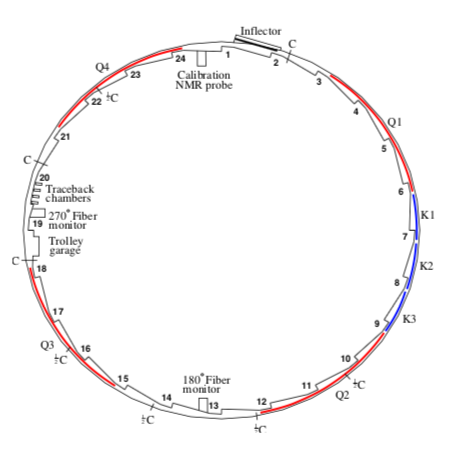
\includegraphics[width=.7\textwidth]{VacuumChamberMap}
    \caption[Vacuum chamber map]{A map of the vacuum chambers in E989. K1-K3 show the locations of the kicker magnets, while Q1-Q4 show the locations of the electrostatic quadrupoles. Also shown is the location of the inflector, the two fiber monitors, and one of the tracker stations.}   
    \label{fig:vacmap}
\end{figure}

\subsection{Electrostatic quadrupoles}

There are four electrostatic quadrupoles (quads) located around the ring as shown in \figref{fig:vacmap}, which focus the beam vertically and defocus the beam horizontally. (The magnetic field of the ring serves to restore the beam radially in combination with the electric field.) Just as in the case of the kickers, the quads must be operated in the vacuum. E989 uses electrostatic focusing elements instead of magnetic ones in order to avoid magnetic field gradients which would limit the precision of the magnetic field measurement. Four quads were chosen in order to maximize the symmetry of the beam motion around the ring. The quads occupy 43\% of the ring circumference, leaving space for other elements around the ring. Each quad is made up of two segments, a short segment of 13\textdegree{} and a long segment of 26\textdegree{}. The quads are made out of as little material as possible in order to reduce multiple scattering of decay positrons passing through them. A picture of the quads installed into one of the vacuum chambers is shown in \figref{fig:Quads}. A simulation of the equipotential lines of the quads is shown in \figref{fig:QuadPotential}. The original design of the quads is detailed in \refref{QuadsE821}.

\begin{figure}[]
    \centering
    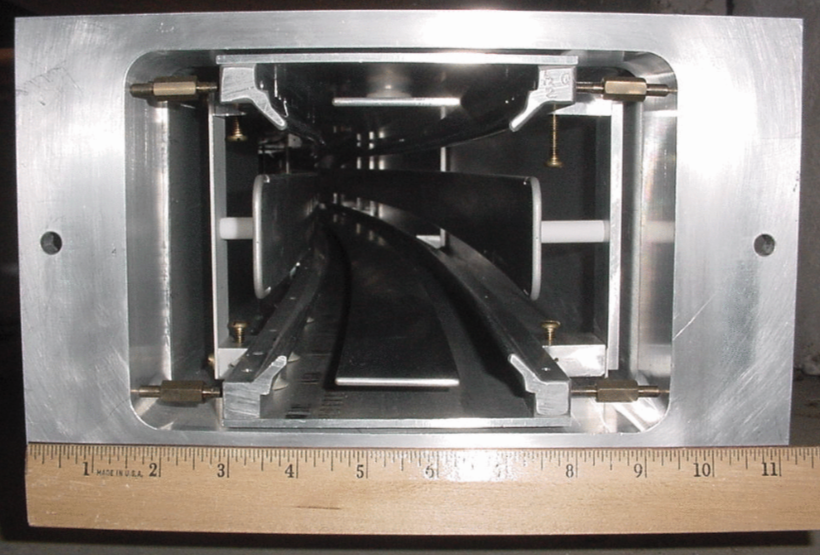
\includegraphics[width=.7\textwidth]{Quads}
    \caption[Electrostatic quadrupoles installed in a vacuum chamber]{Electrostatic quadrupoles installed into a vacuum chamber \cite{QuadsE821}. There are four plates mounted to the chamber through insulator standoffs. Also shown are the rails that the magnetic field trolley rides on around the inside of the ring, and between the quad and kicker plates. The distance between opposing quad plates is $\SI{10}{cm}$.}
    \label{fig:Quads}
\end{figure}

\begin{figure}[]
    \centering
    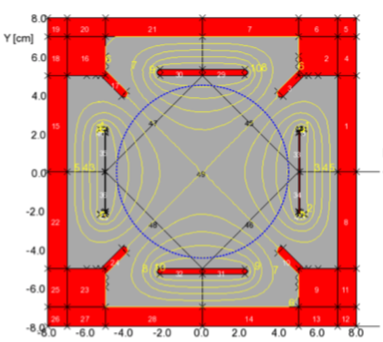
\includegraphics[width=.6\textwidth]{QuadPotential}
    \caption[Electrostatic quadrupole potentials]{An OPERA model of the quads and their equipotential contours. The top and bottom plates sit at positive voltage while the left and right plates are at negative voltage. The muon storage region is shown by the blue circle. Picture from \refref{TDR}.}   
    \label{fig:QuadPotential}
\end{figure}


Lastly, some of the stored muons will be lost during data taking that will affect the measurement of the precession frequency \wa. In order to reduce the number of lost muons over the course of a fill, a procedure called ``scraping'' is used to remove those muons sitting at the edge of the storage region that will likely be lost at later times. This scraping procedure involves powering the quad voltages in an asymmetric way such that the beam is pushed to the outside of the storage region, where the edges of the beam will intersect copper collimators. Muons which hit the collimators will lose energy and be lost as they spiral out of the ring. The scraping procedure is performed early in the fill and ends at \textbf{something}$\SI{20}{\micro s}$. 




\section{Muon beam dynamics}
\label{sec:muonbeamdynamics}

Muons injected into the storage ring will occupy a region in phase space corresponding to a width of momenta and positions. Individual muons will undergo simple harmonic motion or betatron oscillations within the storage ring, in both the vertical and horizontal directions. The strength of the electrostatic focusing in relation to the magnetic field strength can be characterized by the field index
        \begin{align} \label{eq:fieldindex}
            n = \frac{\kappa R_{0}}{\beta B_{0}},
        \end{align}
where $\kappa$ is the electric quadrupole gradient, $B_{0}$ is the magnetic field strength, $R_{0}$ is the central storage ring radius, and $\beta$ is the relativistic velocity of the muon beam. The horizontal and vertical equations of motion, including the effects of the discrete quadrupoles, are given by
        \begin{align} \label{eq:betatronmotion}
            x &= x_{e} + A_{x}(s) \cos(\nu_{x} \frac{s}{R_{0}} + \phi_{x}), \\
            y &= A_{y}(s) \cos(\nu_{y} \frac{s}{R_{0}} + \phi_{y}), 
        \end{align}
where $x_{e}$ is the radial equilibrium orbit of the beam relative to $R_{0}$, $A_{x}(s)$ and $A_{y}(s)$ are the amplitudes of the motions containing the effects of the discreteness of the quads, and $s$ is the arc length of the trajectory. Here $\nu_{x}$ and $\nu_{y}$ are the so-called horizontal and vertical ``tunes'' of the beam motion, which are ratios of the betatron frequencies to the cyclotron frequency. They can be related to the field index $n$ by
        \begin{equation} \label{eq:tunes}
        \begin{aligned}
            \nu_{x} &= f_{x_{BO}}/f_{c} = \sqrt{1-n}, \\
            \nu_{y} &= f_{y_{BO}}/f_{c} = \sqrt{n},           
        \end{aligned}
        \end{equation}
where $f_{c}$ is the cyclotron frequency. Technically $n$ is the the average field index around the ring, where this approximation is justified due to the four-fold symmetry of the discrete quadrupoles and the fact that the betatron oscillations have periods much greater than the length of the quads. A table of the important frequencies in E989 is shown in \tabref{tab:frequencies}. Lastly, the maximum angular acceptance of the ring can be determined from the betatron oscillations and the field index as 
        \begin{equation} \label{eq:maxangles}
        \begin{aligned}
            \psi_{x_{max}} &= \frac{x_{max}\sqrt{1-n}}{R_{0}}, \\
            \psi_{y_{max}} &= \frac{y_{max}\sqrt{n}}{R_{0}},
        \end{aligned}
        \end{equation}
where $x_{max}$ and $y_{max}$ are both equal to the radius of the storage ring aperture at $\SI{45}{mm}$.


\begin{table}[]
\centering
\setlength\tabcolsep{10pt}
\renewcommand{\arraystretch}{1.2}
\begin{tabular*}{1\linewidth}{@{\extracolsep{\fill}}lcccc}
  \hline
    \multicolumn{5}{c}{\textbf{Muon Beam Frequencies}} \\
  \hline\hline
    Name & Symbol & Expression & Frequency (MHz) & Period \\
  \hline
    \gmtwo & $f_{a}$ & $a_{\mu}Be/2\pi m c$ & 0.23 & $\SI{4.365}{\micro s}$ \\
    cyclotron &  $f_{c}$ & $v/\pi R_{0}$ & 6.71 & $\SI{149}{ns}$ \\
    horizontal betatron & $f_{x_{BO}}$ & $\sqrt{1-n} f_{c}$ & 6.34 & $\SI{158}{ns}$ \\
    vertical betatron & $f_{y_{BO}}$ & $\sqrt{n} f_{c}$ & 2.21 & $\SI{452}{ns}$ \\
    coherent betatron & $f_{CBO}$ & $f_{c}-f_{x_{BO}}$ & 0.37 & $\SI{2.703}{\micro s}$ \\
    vertical waist & $f_{VW}$ & $f_{c}-2f_{y_{BO}}$ & 2.31 & $\SI{433}{ns}$ \\
  \hline
\end{tabular*}
\caption[Muon beam frequencies in the E989 experiment]{Frequencies seen in the \gmtwo experiment due to beam motion. Parameter values are from a subset of Run 1 corresponding to an $n$ value of 0.108 or a quad voltage of 18.3 kV.}
\label{tab:frequencies}
\end{table}


As the muon beam goes around the ring, the muons will experience local field gradients and inhomogeneities. The tunes are thus chosen to avoid resonances where muons might be lost from having passed through such perturbations too many times. The muons within the ring should then sample the entire azimuth equally and remain stored. The general resonance condition is \cite{Wiedermann}
        \begin{align}
            a \nu_{x} + b \nu_{y} = c,
        \end{align}
where $a$, $b$, and $c$ are integers. We know from \equref{eq:tunes} that 
        \begin{align}
            \nu_{x}^{2} + \nu_{y}^{2} = 1,
        \end{align}
which constrains the available $n$ values that can be chosen. \figref{fig:tuneplane} shows the space relative to the tunes for which a chosen value of $n$ will lie on a resonance. 

% Moved to Run1 section
% For Run 1 data taking, $n$ values of 0.108 and 0.120 were chosen corresponding to quad voltages of 18.3 and $\SI{20.4}{kV}$ respectively \cite{tunetable}. The associated betatron wavelengths are 1.06 and 3.04 times the circumference of the storage ring respectively.


\begin{figure}[]
    \centering
    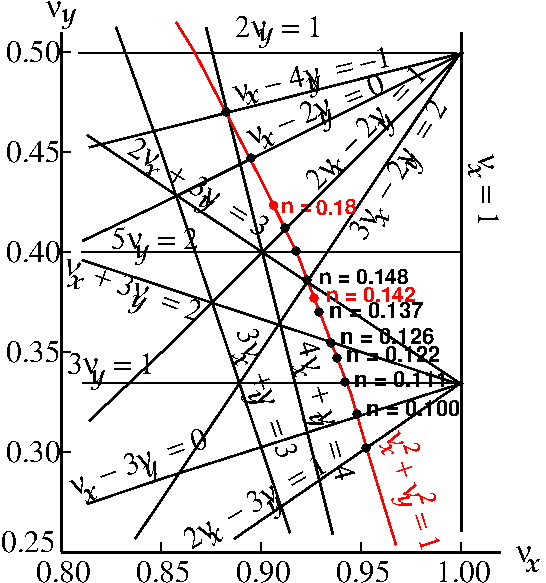
\includegraphics[width=.5\textwidth]{tuneplane}
    \caption[Tune plane]{The tune plane, with the $\nu_{x}^{2} + \nu_{y}^{2} = 1$ constraint in red. The chosen value of $n$ lies on this circle. The original design goals for E989 were the $n$ values as shown by the red points, but due to hardware issues smaller $n$ values of 0.108 and 0.120 were chosen as described in \secref{sec:Run1}.}
    \label{fig:tuneplane}
\end{figure}



\subsection{Coherent betatron oscillation}


With each individual muon undergoing betatron oscillations, the muon beam as a whole will oscillate. The beam can be described as having a width and a mean dependent on the initial phase space parameters determined by injection and kicker effects. This overall distribution of the beam will oscillate coherently every betatron wavelength, thus moving around the ring at some frequency. Individual detectors around the ring measure the beam in discrete pieces based on their individual acceptances, where these acceptances depend on the radial and vertical characteristics of the beam. Because the betatron frequencies are smaller than the cyclotron frequency, there is an aliasing effect such that the betatron motion of the beam is instead observed as an apparent slow-moving oscillation. We call the the measurable signal of this coherent radial motion coherent betatron oscillation (CBO). See \figref{fig:cbo} for a pictorial view of this phenomena. The frequency of the CBO is just the beat frequency between the cyclotron frequency and the horizontal betatron frequency
        \begin{align}
            f_{CBO} = f_{c}-f_{x_{BO}}.
        \end{align}
There is also a horizontal CBO effect, but the rate of oscillation is fast enough that the effect tends to average out. What can be seen in the data however is the vertical width of the beam, to which the detectors are sensitive. Though the principles are the same, we call this effect the vertical waist (VW),
        \begin{align}
            f_{VW} = f_{c}-2f_{y_{BO}},
        \end{align}
where the term waist is used a description of the vertical width when its at its minimum. Both of these frequencies are included in \tabref{tab:frequencies}. For an individual detector the CBO has a specific phase, which goes from \SIrange{0}{2\pi}{} around the ring. When adding all of the detector signals together, the CBO effect tends to cancel out. However, due to acceptance differences between the different detectors, the CBO effect is still observable in the data. When fitting the data to extract \wa, these effects need to be included as will be discussed later.

\begin{figure}[]
    \centering
    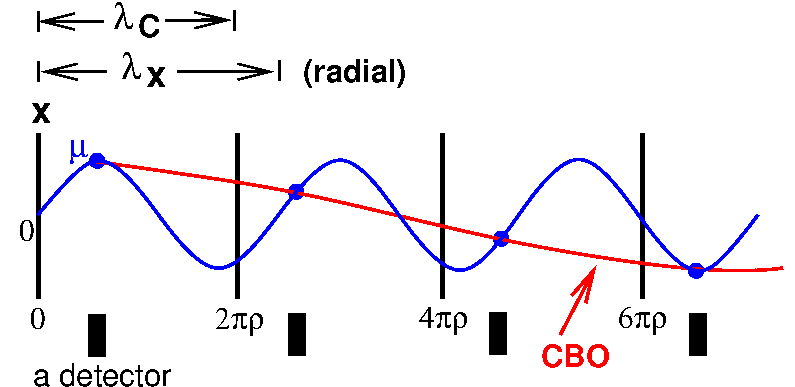
\includegraphics[width=.6\textwidth]{cbo}
    \caption[Coherent betatron oscillation]{Marked by the black vertical lines are integer steps in the circumference of the ring, corresponding to the cyclotron wavelength $\lambda_{c}$. The blue line shows the motion of the beam due to the betatron oscillations $\lambda_{x}$. Since $\lambda_{x} < \lambda_{c}$, there is an aliasing effect in the observed signal, which is identified by the red line. The beam is thus seen as appearing to move back and forth with a slow oscillation, and this is what we call CBO.}
    \label{fig:cbo}
\end{figure}


\subsection{Beam debunching}

As described above, the muon beam is injected into the ring with a time spread of $\SI{120}{ns}$ and a range of momenta. At early times the beam will occupy a portion of the ring less than the whole since the cyclotron period is $\SI{149}{ns}$. Therefore early in the fill the detectors located at discrete points around the ring will measure counts from the beam where there will be a fast oscillation in the signal due to this cyclotron period. As time increases throughout the fill, the momentum distribution of the muons will cause the beam to spread out within the storage ring until the entire azimuth is filled. Since almost all muons are at the same momentum, it turns out that the slower moving muons at smaller radii catch up to the faster moving muons at the outer radii after many turns around the ring. By $\SI{30}{\micro s}$ the muon beam has gone around the ring two hundred times. As the beam fills the storage ring, the cyclotron frequency in the data reduces and the beam is seen to debunch. This phenomena is referred to as the ``fast rotation.'' See \figref{fig:fastrotation} for how this looks in the data. When dealing with the data and attempting to extract \wa, the typical procedure is to both bin out the fast rotation in periods of the cyclotron frequency, and to randomize each hit time by $\pm T_{C}/2$ where $T_{c}$ is the cyclotron period. In this way the fast rotation is removed entirely and the five parameter function described in \equref{eq:5parfunc} remains satisfactory, barring other effects. 

\begin{figure}[]
    \centering
    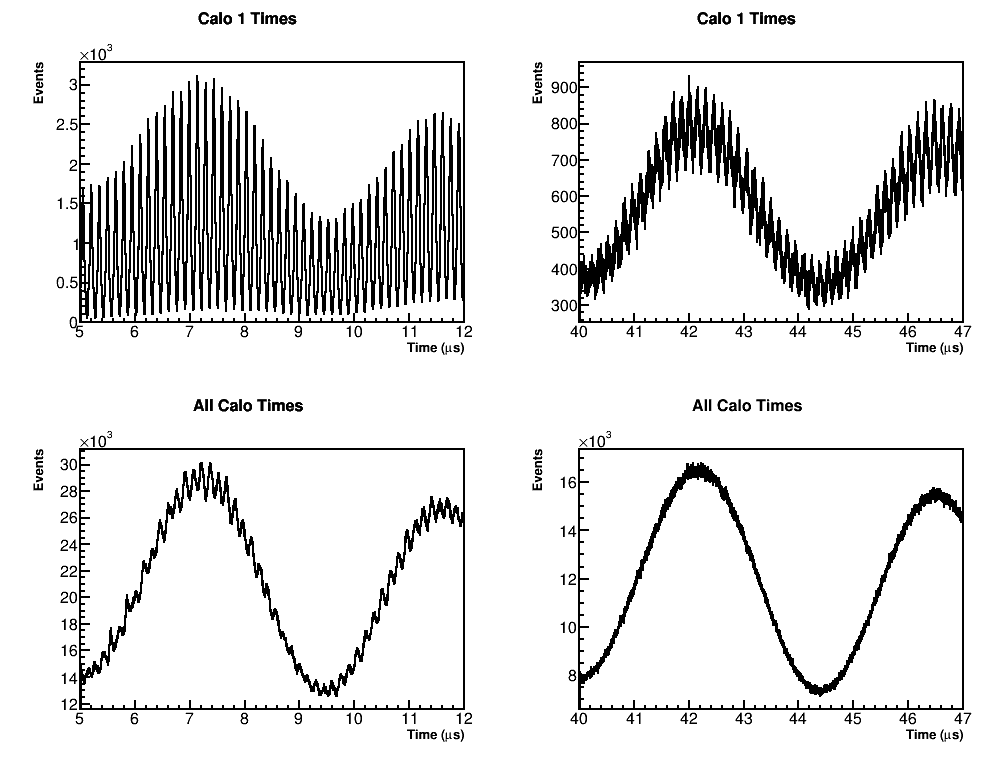
\includegraphics[width=.8\textwidth]{fastrotation}
    \caption[Beam debunching fast rotation]{The fast rotation signal can be seen in the data as an oscillation with a period of $\SI{149}{ns}$, corresponding to the fast oscillations in these plots. In individual calorimeters at early times the fast rotation signal is seen to be very large, as shown on the top left. As time passes and the beam debunches, the amplitude of the fast rotation signal diminishes as shown on the top right. When adding all calorimeters together, the signal reduces as shown in the bottom two plots. In all cases the slow oscillation is the \gmtwo frequency.}
    \label{fig:fastrotation}
\end{figure}



\section{Corrections to \texorpdfstring{\wa}{wa}}

\equref{eq:wasimple} is an idealized version of the spin difference frequency. Including practical experimental concerns, there are two corrections that must be applied to \wa.

\subsection{Electric field correction}
\label{sub:electric_field_correction}

In the presence of an electric field, the spin difference frequency is altered to 
        \begin{align} \label{eq:waelectric}
            \vec{\omega}_{a} = -\frac{q}{m} [a\vec{B} - \Big(a - \frac{1}{\gamma^{2}-1}\Big)(\vec{\beta} \times \vec{E}) ],
        \end{align}
where now there is an extra term dependent on the electric field strength and the momentum of the particles. This is necessary to include since we use electrostatic quadrupoles for vertical focusing as described above. The second term cancels to first order for a specific momentum or value of $\gamma$. This "magic momentum" can be understood as the momentum at which a relativistic particle moving through an electric field has its spin exactly follow its momentum. This magic momentum is $\SI{3.094}{\GeV}$ for muons, hence the momentum value of the injected muons. This value has driven many of the design constraints of the \gmtwo experiment, including the size of the storage ring, choice of the magnetic field magnitude, and so on.

Not all muons will have the magic momentum however as described in the \secref{sec:Accelerator}, and therefore a correction to the measured \wa frequency needs to be applied. Approximating the storage ring as having an electric field applied over the whole azimuth of the ring, the spin difference frequency for muons with momentum $p \neq p_{m}$ (where $p_{m}$ is the magic momentum) becomes  
        \begin{align} \label{eq:waEfield}
            \omega_{a}' = \omega_{a} \Big[ 1 - \beta \frac{E_{r}}{c B_{y}} \Big( 1 - \frac{1}{a \beta^{2} \gamma^{2}} \Big) \Big].
        \end{align}
Here the motion of the beam is assumed purely azimuthal. This additional term is the electric field correction that then serves to lower the measured \wa frequency. Using the relation $p = \beta \gamma m = (p_{m} + \Delta p)$, after a little bit of simplification the electric field correction can be written as
        \begin{align}
            C_{\text{E}} = \frac{\Delta\omega_{a}}{\omega_{a}} = -2 \frac{\beta E_{r}}{c B_{y}} \frac{\Delta p}{p_{m}}.
        \end{align}
The last fraction can be related to the field index described in \equref{eq:fieldindex} by
        \begin{align}
            \frac{\Delta p}{p_{m}} = (1-n) \frac{\Delta R}{R_{0}} = (1-n) \frac{x_{e}}{R_{0}}, 
        \end{align}
since we know that the magic momentum muons live at the center of the storage ring radius $R_{0}$. In this equation $x_{e} = \Delta R$ is the equilibrium radius of the beam relative to the central storage radius. Noting that the electric field strength is 
        \begin{align}
            E = \kappa x = \frac{n \beta c B_{y}}{R_{0}} x,
        \end{align}
and assuming that it is perfectly radial, the electric field correction can be reduced to 
        \begin{align}
            C_{\text{E}} = -2n (1-n) \beta^{2} \frac{x x_{e}}{R_{0}^{2}}.
        \end{align}
Taking the time average of the beam motion, where $x$ is simply equal to $x_{e}$, then the correction becomes
        \begin{align}
            C_{\text{E}} = -2n (1-n) \beta^{2} \frac{\langle x_{e}^{2} \rangle}{R_{0}^{2}}.
        \end{align}
This electric field correction can be determined through analysis which relates the beam momentum to the equilbrium radius. (Should I expand on that somehow here?) The assumptions made here are sufficient for the \gmtwo measurement \cite{something}.


\subsection{Pitch correction}
\label{sub:pitch_correction}

Particles injected into the \gmtwo storage ring will have some motion component that is vertical, or parallel to the magnetic field vector (hence the need for vertically focusing electrostatic quadrupoles). This will reduce the magnetic field seen by the muons in their rest frame slightly. Including this motion into the spin difference frequency (along with the electric field correction describe previously), \wa becomes
        \begin{align} \label{eq:wafinal}
            \vec{\omega}_{a} = -\frac{q}{m} [a\vec{B} - a \Big(\frac{\gamma}{\gamma+1}\Big)(\vec{\beta} \cdot \vec{B})\vec{B} - \Big(a - \frac{1}{\gamma^{2}-1}\Big)(\vec{\beta} \times \vec{E}) ],
        \end{align}
where now there is an extra term in the middle dependent on the vertical betatron motion of the beam. Similar to the electric field case, this term can be neglected to first order as the muon momentum is nearly all perpendicular to the field, but a correction again needs to be applied to \wa to account for this effect.

\begin{figure}[]
    \centering
    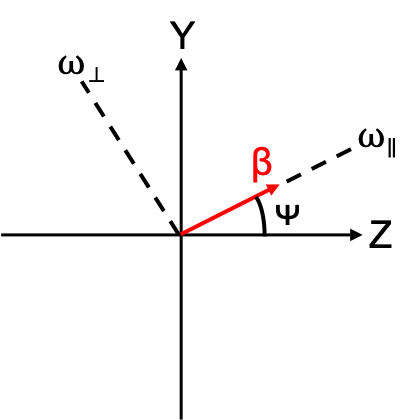
\includegraphics[width=.4\textwidth]{PitchAxes}
    \caption[Pitching beam motion]{Beam motion $\beta$ relative to the vertical and azimuthal axes Y and Z respectively. $\psi$ is the pitch angle of the beam, and the dashed lines represent the parallel and perpendicular motions of the beam.}   
    \label{fig:PitchAxes}
\end{figure}

Since the muons in the storage ring will be oscillating vertically as they are focused by the quads, their momentum vectors will be pitching up and down relative to the azimuthal motion. This pitch angle will oscillate as
        \begin{align} \label{eq:psi}
            \psi = \psi_{0} \cos(\omega_{y}t),
        \end{align}
where $\psi_{0}$ is the amplitude of the oscillation and $\omega_{y}$ is the vertical betatron frequency. Shown in \figref{fig:PitchAxes} is an exaggerated example of the beam motion relative to the vertical and azimuthal axes. Assuming that the field is purely vertical, $\vec{B} = B_{y}\hat{y}$ and that the beam motion is in the vertical-azimuthal plane,
        \begin{align}
            \vec{\beta} = \beta_{y}\hat{y} + \beta_{z}\hat{z} = \beta\cos(\psi)\hat{y} + \beta\sin(\psi)\hat{z},
        \end{align}
then \wa becomes
        \begin{align}
            \vec{\omega}_{a} = -\frac{q}{m} [a B_{y} \hat{y} - a \Big(\frac{\gamma}{\gamma+1}\Big) \beta_{y}B_{y} (\beta\cos(\psi)\hat{y} + \beta\sin(\psi)\hat{z})],        
        \end{align}
where in this case the electric field part has been ignored. Using the small angle approximation such that $\cos(\psi) \approx 1$ and $\sin(\psi) \approx \psi$, $\vec{\omega}_{a}$ can be separated into its vertical and azimuthal components
        \begin{align}
            \omega_{ay} &= \omega_{a}\Big[ 1 - \Big(\frac{\gamma-1}{\gamma}\Big) \psi^{2} \Big], \\     
            \omega_{az} &= -\omega_{a} \Big(\frac{\gamma-1}{\gamma}\Big) \psi.
        \end{align}
Looking at \figref{fig:PitchAxes} again, it can be seen that the spin difference frequency can be resolved into its parallel and perpendicular components $\omega_{\parallel}$ and $\omega_{\perp}$ respectively. As the pitch angle of the beam motion oscillates about the azimuthal axes at a frequency much greater than the \gmtwo frequency, it can be seen that the parallel component averages to 0 over time. (Haven't given a number for the vertical betatron frequency yet.) We then only care about the perpendicular oscillation of the beam, which can be determined with a simple rotation matrix such that
        \begin{align}
            \omega_{a} \approx \omega_{\perp} = \omega_{ay} \cos(\psi) - \omega_{az}\sin(\psi) \approx \omega_{a} \Big[ 1 - \frac{\psi^{2}}{2} \Big],
        \end{align}
where in the last approximation the small angle approximation was used once again, but this time with $\cos(\psi) \approx 1 - \psi^{2}/2$. The pitch correction then is the additional term which serves to lower the measured spin difference frequency. Taking the time average,
        \begin{align}
            C_{\text{P}} = \frac{\Delta\omega_{a}}{\omega_{a}} = - \frac{\langle \psi^{2} \rangle}{2} = - \frac{\langle \psi_{0}^{2} \rangle}{4},
        \end{align}
where \equref{eq:psi} was used in the last equality. The pitch angle of the beam cannot be measured directly, however we know from \equref{eq:maxangles} that the angle of the beam can be related to the vertical distribution of the beam, such that 
        \begin{align}
            C_{\text{P}} = - \frac{n}{4} \frac{\langle y^{2} \rangle}{R_{0}^{2}}.
        \end{align}
Once again $n$ is the field index, $R_{0}$ is the radius of the ring at the center of the storage region, and $\langle y^{2} \rangle$ is the vertical width of the beam. The first two are known and the last can be measured experimentally. (For this last equation make sure that what I write here gels with what I'll put in other sections, which haven't been done yet.) While this derivation was an approximation assuming continuous quads around the ring, it suffices for the level of precision necessary for the \gmtwo experiment \cite{something}.



\section{Run 1 in E989}
\label{sec:Run1}


Run 1 for E989 was conducted in the first half of 2018. Production data was gathered from March 22nd through June 29th. Because of accelerator, experimental, and practical concerns production data taking was interrupted at various dates. Due to hardware issues both kicker and quad settings were lowered from their original design values. Stable voltage set points were identified and used in separate periods of the data taking, depending on the stabilities of the systems. The distinct datasets and their associated parameters are shown in \tabref{tab:Run1Datasets}. For Run 1, $n$ values of 0.108 and 0.120 were chosen corresponding to quad voltages of 18.3 and $\SI{20.4}{kV}$ respectively \cite{tunetable}. The associated betatron wavelengths are 1.06 and 3.04 times the circumference of the storage ring respectively.




From kicker section:
In Run 1 the kickers were not able to be run at the design voltage necessary to put the beam exactly on the central orbit. Instead the beam is kicked to a stable orbit a couple of mm off center depending on the actual value of the kick used, as shown in \figref{fig:BeamCrossSection}. \textbf{(Clarify what the exact numbers are here, or point to the section where I describe the values used in Run 1.)}  


From quad section:
During Run 1 it was discovered that some of the quad resistors were damaged, leading to longer RC time constants such that the quad voltages had not returned to storage nominal during the designated analysis portion of the data. \textbf{(Show a picture here of those time constants?)} Note that despite this scraping procedure, some stored muons are still lost anyways. The effects on the measurement of \wa due to this are explored in \secref{sec:lostmuons}.



-number of muons per fill number somewhere...
% Kiburg 13699
% Polly 12936 but neither of these quite give the actual number of muons per fill



\cite{Run1Datasets}




\begin{landscape}
\begin{table}[]
\centering
\setlength\tabcolsep{10pt}
\renewcommand{\arraystretch}{1.2}
\begin{tabular*}{1\linewidth}{@{\extracolsep{\fill}}lccccc}
  \hline
    \multicolumn{6}{c}{\textbf{Run 1 Datasets}} \\
  \hline\hline
    Name & Number $e^{+} > E_{\text{Th}}$ & $n$ Value & Quad Voltage (kV) & Kicker Voltage Range (kV) & $f_{CBO}$ (MHz) \\
  \hline
    60H & $\SI{9.3e8}{}$ & 0.108 & 18.3 & \SIrange{128}{132}{} & 0.37 \\
    HighKick &  & 0.120 & 20.4 & \SIrange{136}{138}{} &  \\
    9d & $\SI{2.2e9}{}$ & 0.120 & 20.4 & \SIrange{128}{132}{} &  \\
    LowKick &  & 0.120 & 20.4 & \SIrange{123}{127}{} &  \\
    SuperLowKick & & 0.108 & 18.3 & \SIrange{117}{119}{} &  \\
    Endgame &  & 0.108 & 18.3 & \SIrange{122}{127}{} &  \\
  \hline
    % Total Positrons Above Threshold
  \hline
\end{tabular*}
\caption[Run 1 datasets]{ \textbf{Update the number of positrons column once all of the datasets have been opened and energy thresholds chosen. Potentially also add further columns of interest or split into multiple tables.}}
\label{tab:Run1Datasets}
\end{table}
\end{landscape}





\cleardoublepage




